\documentclass[a4j]{jarticle}
\usepackage{graphicx}
\usepackage[left=25truemm,right=25truemm]{geometry}

\title{画像処理 レポート}

\author{氏名: 木下直樹\\学籍番号: 09425521}

\date{提出日: 2015月11月30日}

\begin{document}
\maketitle

%%%%%%%%%%%%%%%%%%%%%%%%%%%%%%%%%%%%%%%%%%%%%%%%%%
\section{概要}
%%%%%%%%%%%%%%%%%%%%%%%%%%%%%%%%%%%%%%%%%%%%%%%%%%
画像の特徴点を自動検出させるためにTKfilter.cを作成する.
計算部であるImageFeature()を完成させ, 可能であればその計算を最適化させる. 

%%%%%%%%%%%%%%%%%%%%%%%%%%%%%%%%%%%%%%%%%%%%%%%%%%
\section{ImageFeature()の作成}
%%%%%%%%%%%%%%%%%%%%%%%%%%%%%%%%%%%%%%%%%%%%%%%%%%
以下のようなコードを作成した.

\begin{verbatim}
 void ImageFeature(Matrix*im2,Image*im){
  int x,y,u,v,W=7,ix,iy;
  double a;
  for(y=W+1;y<im->H-W-1;y++) for(x=W+1;x<im->W-W-1;x++){
    double ixx,ixy,iyy;
    ixx=iyy=ixy=0;
    for(v=-W;v<=W;v++) for(u=-W;u<=W;u++){
      ix=IElem(im, x+u+1, y+v, 1) - IElem(im, x+u-1, y+v, 1);
      iy=IElem(im, x+u, y+v+1, 1) - IElem(im, x+u, y+v-1, 1);
      ixx+=ix*ix;
      ixy+=ix*iy;
      iyy+=iy*iy;
    }
    a=((ixx+iyy)-sqrt(pow(ixx+iyy,2)-4*(ixx*iyy-pow(ixy,2))))/2;
    DElem(im2,x,y)=a; // 実際には [ixx,ixy;ixy,iyy] の小さい方の固有値を入れる.
  }
}
\end{verbatim}

出力結果は以下である.\\
\begin{center}
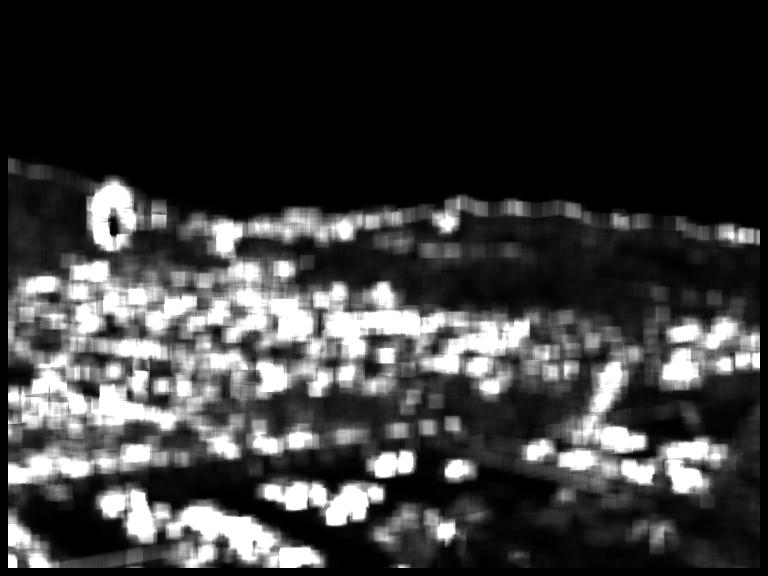
\includegraphics[bb=0 0 768 576,scale=.35]{out.jpg}
\end{center}
このプログラムでは特徴点検出に多くの計算時間を要してしまう. 
そのため, その計算部の効率化が望まれる. 
そこで, その計算に対してGPUによる処理を適用した. 
以下はそのコードである. 
{\baselineskip 2mm
\begin{verbatim}
#include"image.h"
#define getpix(x,y) img[((x)+imW*(y))*3+1]

__global__ void gpuTK_vertical(float*tmp,unsigned char *img,int imW,int imH){
  int x=blockDim.x*blockIdx.x+threadIdx.x;
  int y=blockDim.y*blockIdx.y+threadIdx.y;
  int v,W=7;
  int mat=imW*imH;

  if(W+1<=y && y<imH-W-1)
    if(1<=x && x<imW-1){
      float ix,iy,ixx,ixy,iyy;
      ixx=iyy=ixy=0;
      for(v=-W;v<=W;v++){
	ix=getpix(x+1,y+v)-getpix(x-1,y+v);
	iy=getpix(x,y+v+1)-getpix(x,y+v-1);
	ixx+=ix*ix;
	ixy+=ix*iy;
	iyy+=iy*iy;
      }
      tmp[(x+imW*y)]=ixx;
      tmp[(x+imW*y+mat)]=ixy;
      tmp[(x+imW*y+mat*2)]=iyy;
    }
}

__global__ void gpuTK_horizontal(double*fimg,float*tmp,int imW,int imH){
  int x=blockDim.x*blockIdx.x+threadIdx.x;
  int y=blockDim.y*blockIdx.y+threadIdx.y;
  int u,W=7;
  int mat=imW*imH;

  if(W+1<=y && y<imH-W-1 &&
     W+1<=x && x<imW-W-1){
      float ixx,ixy,iyy;
      double lamd;
      ixx=iyy=ixy=0;
      for(u=-W;u<=W;u++){
	ixx+=tmp[(x+u+imW*y)];
	ixy+=tmp[(x+u+imW*y+mat)];
	iyy+=tmp[(x+u+imW*y+mat*2)];
      }
      lamd=((ixx+iyy)-sqrt(pow(ixx+iyy,2)-4*(ixx*iyy-ixy*ixy)))/2;
      fimg[x+imW*y]=lamd;
    }else fimg[x+imW*y]=0;
}


typedef struct {
  double *data;
  int W,H;
} Matrix;

// TKfilter.c では ImageFeature 本体を除去して,
// プロトタイプ宣言 void ImageFeature(Matrix*im2,Image*im); のみを書く.

extern "C"
void ImageFeature(Matrix*im2,Image*im){
  double*d_dst;
  float *d_tmp;
  unsigned char*d_src;
  cudaMalloc(&d_src,im->W*im->H*3);
  cudaMalloc(&d_dst,sizeof(double)*im->W*im->H);
  cudaMalloc(&d_tmp,sizeof(float)*im->W*im->H*3);
  cudaMemcpy(d_src,im->data,im->W*im->H*3,cudaMemcpyHostToDevice);
  gpuTK_vertical<<<dim3((im->W+15)/16,(im->H+15)/16),dim3(16,16)>>>(d_tmp,d_src,im->W,im->H);
  gpuTK_horizontal<<<dim3((im->W+15)/16,(im->H+15)/16),dim3(16,16)>>>(d_dst,d_tmp,im->W,im->H);  
  cudaMemcpy(im2->data,d_dst,im->W*im->H*sizeof(double),cudaMemcpyDeviceToHost);
  cudaFree(d_dst);
  cudaFree(d_src);
  cudaFree(d_tmp);
}
\end{verbatim}
}

これを適用したことにより, 特徴点検出にかかる計算時間は以下の様に改善された. 

\begin{tabular}{|l|c|c|}
  \hline
  & 改善前(GPU不使用の単純処理) & 改善後(GPUによる処理を採用)\\
  \hline
  時間 & 242 msec & 4.3 msec\\
  \hline
\end{tabular}

\end{document}
